%*******************************************************************************
%****************************** Second Chapter *********************************
%*******************************************************************************
\nomenclature[z-ARM]{ARM}{Advanced RISC Machine}
\nomenclature[z-Rpi1]{Rpi}{Raspberry Pi  Modello B}
\nomenclature[z-Rpi2]{Rpi2}{Raspberry Pi 2}
\nomenclature[z-Rpi3]{Rpi3}{Raspberry Pi 3}
\nomenclature[z-CLR]{CLR}{Common Language Runtime}
\nomenclature[z-CL]{CL}{Common Language}
\nomenclature[z-GPU]{GPU}{Graphics Processing unit}
\nomenclature[z-CPU]{CPU}{Central Processing unit}
\nomenclature[z-SoC]{SoC}{System-On-Chip}
\nomenclature[z-GPIO]{GPIO}{General Purpose Input/Output}
\nomenclature[z-ML]{ML}{MetaLanguage, Functional Language}
\nomenclature[z-NPM]{NPM}{Node.js Package Manager}
\nomenclature[z-USB]{USB}{Universal Serial BUS}
\nomenclature[z-IOT]{IoT}{Internet Of Things}
\chapter{Preliminari}

\ifpdf
    \graphicspath{{Chapter2/Figs/Raster/}{Chapter2/Figs/PDF/}{Chapter2/Figs/}}
\else
    \graphicspath{{Chapter2/Figs/Vector/}{Chapter2/Figs/}}
\fi


\section{Raspberry Pi}

Il Raspberry Pi è un calcolatore  a basso costo  di dimensioni molto ridotte realizzato dalla RaspberryPi Fondantion, di questo piccolo computer esistono diverse versioni con configurazioni hardware differenti così come riportato dalla tabella \ref{tab:rpi_ver}.

\begin{figure}[htbp!] 
	\centering    
	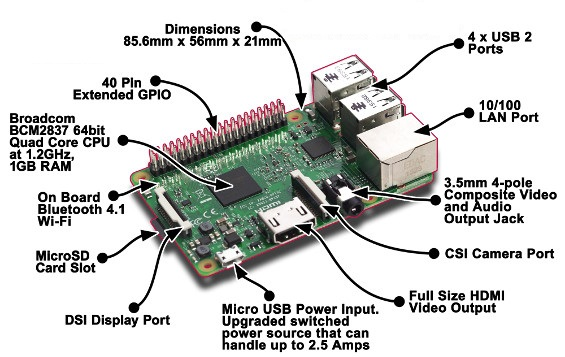
\includegraphics[width=1.0\textwidth]{rpi3}
	\caption[RaspberryPi 3]{Raspberry Pi 3}
	\label{fig:rpi3}
\end{figure}

\begin{landscape}
\begin{table}[htbp]
	\caption{Comparazione modelli Raspberry Pi}
	\begin{tabular}{|l|c|c|c|c|}
		\hline
		\multicolumn{1}{|c|}{\textbf{Modello}} & \textbf{Rpi} & \textbf{Rpi2} & \textbf{Rpi2 v1.2} & \textbf{Rpi3} \\ \hline
		Data di introduzione & 2014-07-01 & 2015-02-01 & 2016-10-01 & 2016-02-01 \\ \hline
		Processore SoC & Broadcom BCM2835 & Broadcom BCM2836 & \multicolumn{ 2}{c|}{Broadcom BCM2837} \\ \hline
		Architettura & ARMv6Z (32 bit) & ARMv7-A (32 bit) & \multicolumn{ 2}{c|}{ARMv8-A (32/64 bit)} \\ \hline
		CPU & ARM11 & ARM Cortex A7 & \multicolumn{ 2}{c|}{ARM Cortex A53} \\ \hline
		Numero di core & 1 & 4 & 4 & 4 \\ \hline
		Frequenza CPU (Mhz) & 700 & \multicolumn{ 2}{c|}{900} & 1200 \\ \hline
		GPU & \multicolumn{ 4}{c|}{Broadcom VideoCore IV} \\ \hline
		Memoria SDRAM & 512 & \multicolumn{ 3}{c|}{1024} \\ \hline
		Porte Usb 2.0 & 4 &  &  &  \\ \hline
		Input video & \multicolumn{ 4}{c|}{Connettore 15-pin MIPI  CSI usato con la Raspberry Pi camera} \\ \hline
		Output Video & \multicolumn{ 4}{l|}{HDMI (rev 1.3), video composito TRRS 3.5 jack, MIPI display interface DSI per pannelli LCD} \\ \hline
		Input Audio & \multicolumn{ 4}{c|}{su board attraverso porte I2S} \\ \hline
		Output Audio & \multicolumn{ 4}{c|}{analogico via jack 3.5mm, digitale via HDMI e su board I2S} \\ \hline
		Storage Slot & SD & \multicolumn{ 3}{c|}{MicroSDHC} \\ \hline
		Ethernet & \multicolumn{ 4}{c|}{10/100 Mbit/s} \\ \hline
		Wi-Fi & \multicolumn{ 3}{c|}{no} & 802.11n wireless \\ \hline
		Bluetooth & \multicolumn{ 3}{c|}{no} & Bluetooth 4.1 \\ \hline
		GPIO & \multicolumn{ 4}{c|}{17× GPIO plus the same specific functions, and HAT ID bus } \\ \hline
		Alimentazione & 600mA (3.0W) & \multicolumn{ 3}{c|}{800 mA(4.0 W)} \\ \hline
		dimensione & \multicolumn{ 4}{c|}{85.60 mm × 56.5 mm } \\ \hline
		Peso  & \multicolumn{ 4}{c|}{45g} \\ \hline
	\end{tabular}
	
	\label{tab:rpi_ver}
\end{table}
\end{landscape}

La scelta per il progetto oggetto di questa tesi è stata per Raspeberry 3, che indicherò da questo momento come Rpi3, perchè mette a disposizione una potenza di calcolo superiorie a qualunche altro modello di RPi.

Questa versione è dotata di un  SoC BCM2837  dove all'interno del quale c'è:
\begin{itemize}
	\item CPU quad-core ARM Cortex A53 4 bit a 1.2 Ghz,
	\item 1 GB SDRAM di memoria, e
	\item GPU VideoCore IV a 400Mhz
\end{itemize}
inoltre  è dotato del chip BCM43438 che fornisce connettività Wifi b/g/n e Bluetooth eliminando la necessità di utilizzare  adatattori Wifi USB, e come nelle precedenti versioni sono presenti 17 pin GPIO, dove è possibile controllare dispostivi aggiuntivi, e l'interfaccia CSI, che consente di collegare una periferica di input video. 

Il piccolo calcolatore dalle dimensioni di una carta di credito, come può essere visto in \figurename~\ref{fig:rpi3}, ha l'antenna usata per le comunicazioni wireless sul bordo esterno della scheda, fuori dalla portata di possibili interferenze causate  da eventuali dispositivi e componenti aggiuntivi. 

L'integrazione delle comunicazioni wireless insieme alla possibilità di collegare periferiche e componenti aggiuntivi lo rende interessante per essere una piattaforma si sviluppo di un sistema IoT.

Tra le altre caratteristiche interessanti di questo computer è  la presenza di  quattro porte USB e una porta Ethernet 10/100 che condividono lo stesso bus gestito dal chip LAN9514. 
Questa soluzione può essere criticata  perchè non permette di sfruttare il 1 Gbit sulla porta Ethernet, ma ai fini del nostro progetto non è un difetto che penalizza la sua realizzazione.

Nel dispositivo non è presente nessun tipo di memoria di massa, ma è presente un lettore di memorie MicroSD.
L'avvio del sistema avviene dalla scheda MicroSD dove all'interno c'è una partizione con sopra il firmware, kernel e la configurazione del sistema.

Questo calcolatore è stato progettato per funzionare con diversi sistemi operativi Linux, RiscOS e Windows Core Iot.

Per questo progetto su Rpi3 installerò Linux Raspian, una distribuzione Linux pensata per Raspberry.



\subsection{GPIO}
In Rpi3 sono presenti 54 linee GPIO di queste linee molto sono riservate ai diversi componenti presenti nella scheda  come il lettore di schede microSD, l'uscita audio, ingresso CSI,uscita DSI e i vari LED di stato.

I GPIO che interessano di più sono quelli che si trovano nel pettine da 40 pin, visibile sulla scheda su due linee da 20, che forniscono il supporto per SPI, I2C, PWM e UART Seriale.
La numerazione di questi pin avviene dall'alto in basso e da sinistra a destra e il primo P1 viene scritto sulla scheda per facilitarne l'individuzione.
Inizialmente tutti i pin sono impostati a GPIO a parte i GPIO 14 e GPIO 15 che sono inizializzati per l'utilizzo di UART, ma via software anche questi possono essere riconfigurati a GPIO, in totale possono essere utilizzati 17 GPIO.
Per motivi di architettura, la numerazione GPIO utilizzata dalle librerie di accesso ai pin è differente rispetto alla numerazione dei pin, quindi è necessario fare riferimento alla \figurename~\ref{fig:gpio-map} per individuare il pin associato, inoltre bisogna fare attenzione a lavorare con queste linee perchè richiedono 3.3 V e non tollerano i 5 volt e quindi collegare qualcosa che immetta 5 volt su un pin GPIO equivale a danneggiare il SoC.

Ogni GPIO supporta gli interrupt che possono essere delle seguenti tipologie:  high, low,  rise,  fall  e  change.   
Non è presente nel kernel ufficiale di Linux la possibilità di utilizzare questi interrupt ma esiste una una patch che li abilita.
Per poter sfruttare gli interrupt GPIO senza applicare le patch al kernel utilizzerò la distribuzione Raspbian che include il kernel con il supporto degli interrupt


\begin{figure}[htbp!] 
	\centering    
	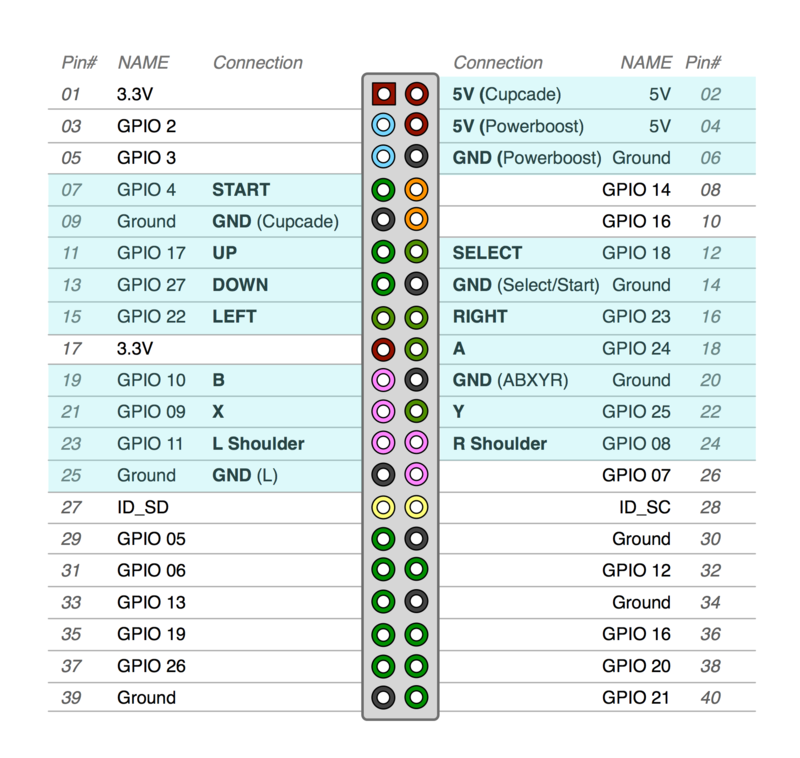
\includegraphics[width=1.0\textwidth]{gpio-map}
	\caption[Mappa GPIO]{La mappa delle Pin GPIO su Raspberry Pi}
	\label{fig:gpio-map}
\end{figure}


\subsection{Raspberry Camera}
Questa camera si collega a Raspberry Pi tramite la porta CSI, come mostrato nella \figurename~\ref{fig:camera} e consente di creare video HD e scattare fotografie digitali, ha integrato il sensore di immagine CMOS IMX219PQ Sony da 8 megapixel ad alta qualità ed elevata sensibilità, con funzioni di video imaging ad alta velocità e supporto delle modalità video 1080p30, 720p60 e VGA90.
Esis
\begin{figure}[htbp!] 
	\centering    
	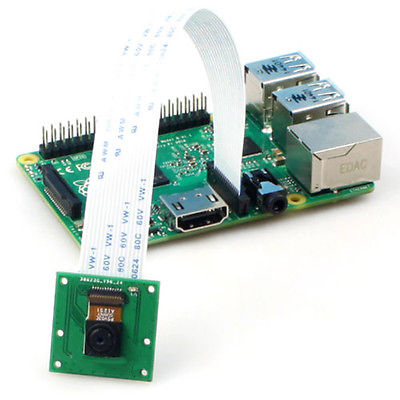
\includegraphics[width=1.0\textwidth]{cam_csi}
	\caption[Raspberry Camera]{La Raspberry Camera}
	\label{fig:camera}
\end{figure}
In Raspian sono presenti comandi che permettono di utilizzare la Raspberry Camera:
\begin{itemize}
	\item \texttt{rasp-config} è lo strumento di configurazione  Raspberry Pi che permette di abilitare l'interfaccia CSI per l'uso della Raspberry Camera,
	\item \texttt{raspstill} è un comando che cattura delle fotografie con il modulo telecamera e lo salva su un file,
	\item \texttt{raspvid} permette di registrare un video e salvarlo su un file.
\end{itemize}
Il primo comando rasp-config va lanciato soltanto la prima volta in fase di configurazione del sistema per abilitare la camera, mentre raspstill e raspvid verranno utilizzati nel progetto per acquisire immagini e filmati.

\subsection{L298N Motor Controller}
Si tratta di un modulo elettronico basato appunto sull’integrato L298, e sarà utilizzato per pilotare motori.

\begin{figure}[htbp!] 
	\centering    
	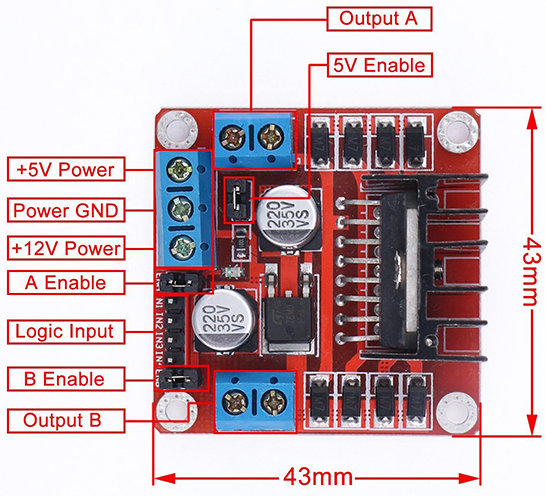
\includegraphics[width=1.0\textwidth]{L298N}
	\caption[L298N Motor Controller]{L298N Motor Controller}
	\label{fig:L298N}
\end{figure}
Così come mostrato dalla \figurename~\ref{fig:L298N}, questo circuito è composto da due connettori laterali ai quali collegare i motori, e da connettori frontali dove collegare l’alimentazione e le connessioni logiche necessarie a controllare i carichi.

\begin{figure}[htbp!] 
	\centering    
	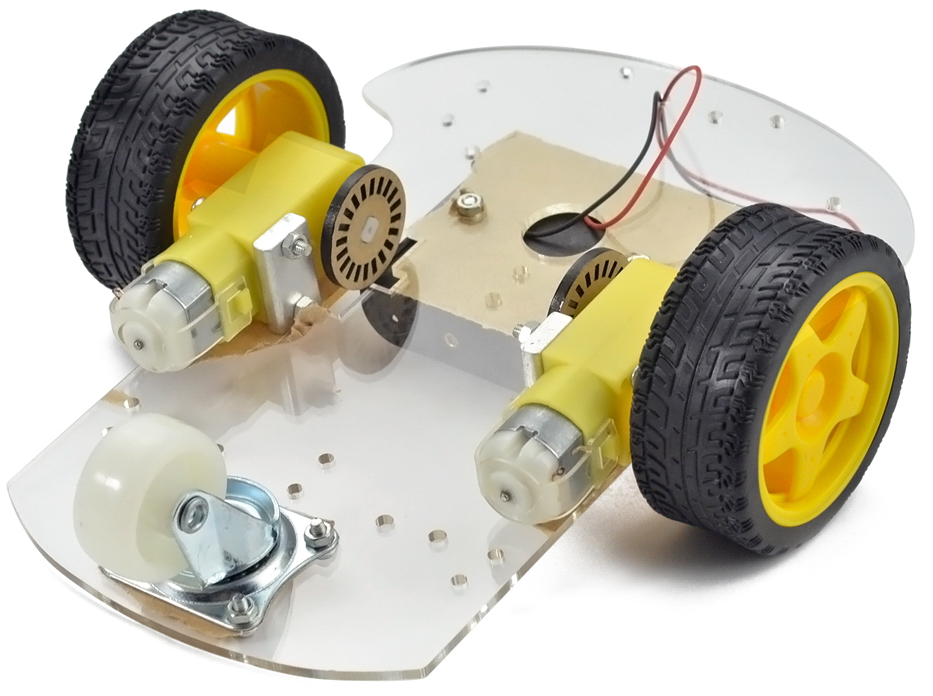
\includegraphics[width=1.0\textwidth]{chassis}
	\caption[Rover Chassis]{Rover Chassis con ruote, vano batteria}
	\label{fig:chassis}
\end{figure}
Questo modulo sarà collegato nel progetto finale direttamente allo chassis, \figurename~\ref{fig:chassis}, dove saranno presenti i motori e il vano batteria.


\subsection{HC-SR04}


Il  sensore ad ultrasuoni HC-SR04 emette un impulso ad ultrasuoni e calcola il tempo impiegato dall’impulso per raggiungere il primo ostacolo di fronte a lui e tornare indietro.


\begin{figure}[htbp!] 
	\centering    
	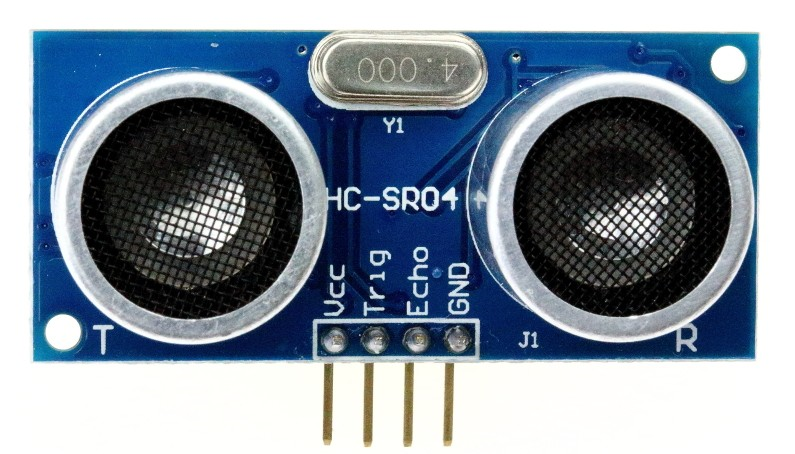
\includegraphics[width=1.0\textwidth]{hc-sr04}
	\caption[HC-SR04]{Il sensore ad ultrasuoni hc-sr04}
	\label{fig:hc-sr04}
\end{figure}
Come si può vedere dalla \figurename~\ref{fig:hc-sr04} Il sensore oltre essere composto dalle l'emittitore e dal recevitore dispone di 4 pin:
\begin{itemize}
 \item Vcc (+5V), 
 \item Trigger, 
 \item Echo, 
 \item GND. 
\end{itemize}

Il funzionamento del sensore avviene in questo modo:
\begin{enumerate}
 \item Si invia un impulso alto sul pin Trigger per almeno 10 microsec,
 \item il sensore invia il ping sonoro e aspetta il ritorno delle onde riflesse,
 \item il sensore risponderà sul pin Echo con un impulso alto della durata corrispondente a quella di viaggio delle onde sonore
\end{enumerate}

Conoscendo velocità di propagazione $ v_{aria} $ del suono nell’aria e  il tempo $t$, che passa dall'invio del segnale al Trigger alla ricezione del segnale Echo, è possibile stabilire la distanza $d_{eo}$ fra il sensore e l’ostacolo  grazie all'equazione della velocità  \[v_{aria} = \dfrac{s}{t} \] dove $s$ è la somma della distanza tra emettitore-oggetto $d_{eo}$ ed della distanza oggetto-ricevitore $d_{or}$ 

Considerando $d_{eo} = d_{or}$ avrò che $s=2 \cdot d_{eo}$ quindi la formula per otterere la distanza sarà 
\[d_{eo} = \dfrac{v_{aria} \cdot t}{2} \]
 

C'è da notare che nell’aria, la velocità del suono è di 331,45 m/s a $0 ^oC$ (pari a 1 193,04 km/h) e di 343,8 m/s (pari a 1 237,68 km/h) a  $20 ^oC$ (e in generale varia secondo la relazione $v_{aria} = 331,45 + 0,62 \cdot v_\delta$ con $v_\delta$ misurata in $^oC$) quindi per semplicità nel corso del progetto ipotizzerò una temperatura di circa $20 ^oC$ quindi una $v_{aria}$ di 343,4 m/s.

quindi la formula sarà
\[d_{eo} = \dfrac{343,8 \cdot t}{2}  \]
 
Se il tempo risulta maggiore di 38 ms si considera che non sia stato incontranto nessun ostacolo e per sicurezza si aspettano 50 ms per far in modo che non siano interferenze con la misura successiva.


%C'è da notare che 

%Si invia un impulso alto sul pin Trigger per almeno 10 microsecondi, a questo punto il sensore invierà il ping sonoro e aspetterà il ritorno delle onde riflesse, il sensore risponderà sul pin Echo con un impulso alto della durata corrispondente a quella di viaggio delle onde sonore, dopo 38 millisecondi si considera che non sia stato incontrato alcun ostacolo.

%Per sicurezza si aspettano in genere 50-60 millisec per far si che non vi siano interferenze con la misura successiva.

\subsection{BreadBoard}
Una breadboard permette di riprodurre il comportamento di un circuito stampato e non richiede saltatura di componenti, è possibile semplicemente inserire i componenti nei fori predisposti sulla board.

\begin{figure}[htbp!] 
	\centering    
	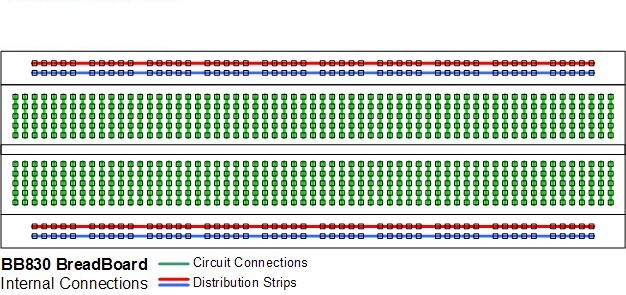
\includegraphics[width=1.0\textwidth]{breadboard}
	\caption[Breadboard]{Breadboard}
	\label{fig:breadboard}
\end{figure}

La breadboard che ho utilizzato ha 830 fori. Come è possibile vedere dalla \figurename~\ref{fig:breadboard}, questo tipo di board ha due linee di punti laterali che corrono per tutta la lunghezza della breadboard ed ogni punto di ogni singola linea è collegato tra loro e queste linee le utilizzerò per l’alimentazione. 

Le linee di punti interne della breadboard invece sono collegati a gruppi di due, i gruppi sono divisi da una scanalatura e ognuno dei quali è composto da 5 punti collegati tra loro.

Tutti i punti della breadboard  hanno una distanza di 2.54mm tra loro e sono contrassegnati da un numero o da una lettera per facilitarne l'uso.

Per facilitare la costruzione e il testing utilizzero un cavo piatto a 40 pin ed un T-cobbler per collegare Rpi3 alla breadboard, in questo modo potrò lavorare con tutti i GPIO direttamente sulla board di test e per collegare i vari componenti userò jumper di vari colori e lunghezze, la \figurename~\ref{fig:t-cobbler-40} mostra questi oggetti. 


\begin{figure}[htbp!] 
	\centering    
	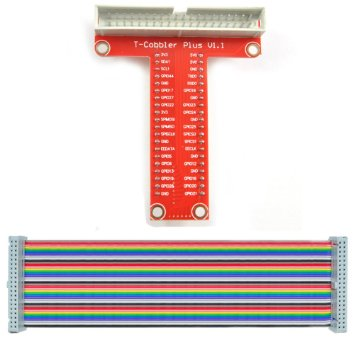
\includegraphics[width=1.0\textwidth]{t-cobbler-40}
	\caption[t-cobbler-40]{I jumper, Cavo 40 Pin e T-Cobbler}
	\label{fig:t-cobbler-40}
\end{figure}


\section{Mono}
Mono è un progetto opensource coordinato da Xamarin, dal 2015 è diventata un'azienda sussidiaria di Microsoft, che ha lo scopo di realizzare  un insieme di strumenti compatibili con il Framework .NET di Microsoft ed aderenti allo standard  ECMA Common Language Infrastructure (CLI)  anche per ambienti non Windows.


La specifica CLI è divisa in quattro parti:
\begin{itemize}
\item Il Common Type System o CTS: un insieme di tipi di dato e di operazioni su di essi.
\item I Metadata: le informazioni sulla struttura del programma. Esse sono indipendenti dal linguaggio di partenza per permettere a programmi scritti in linguaggi differenti di comunicare tra loro.
\item La Common Language Specification o CLS.
\item Il Virtual Execution System o VES: il sistema che esegue i programmi CLI.
\end{itemize}
\begin{figure}[htbp!] 
	\centering    
	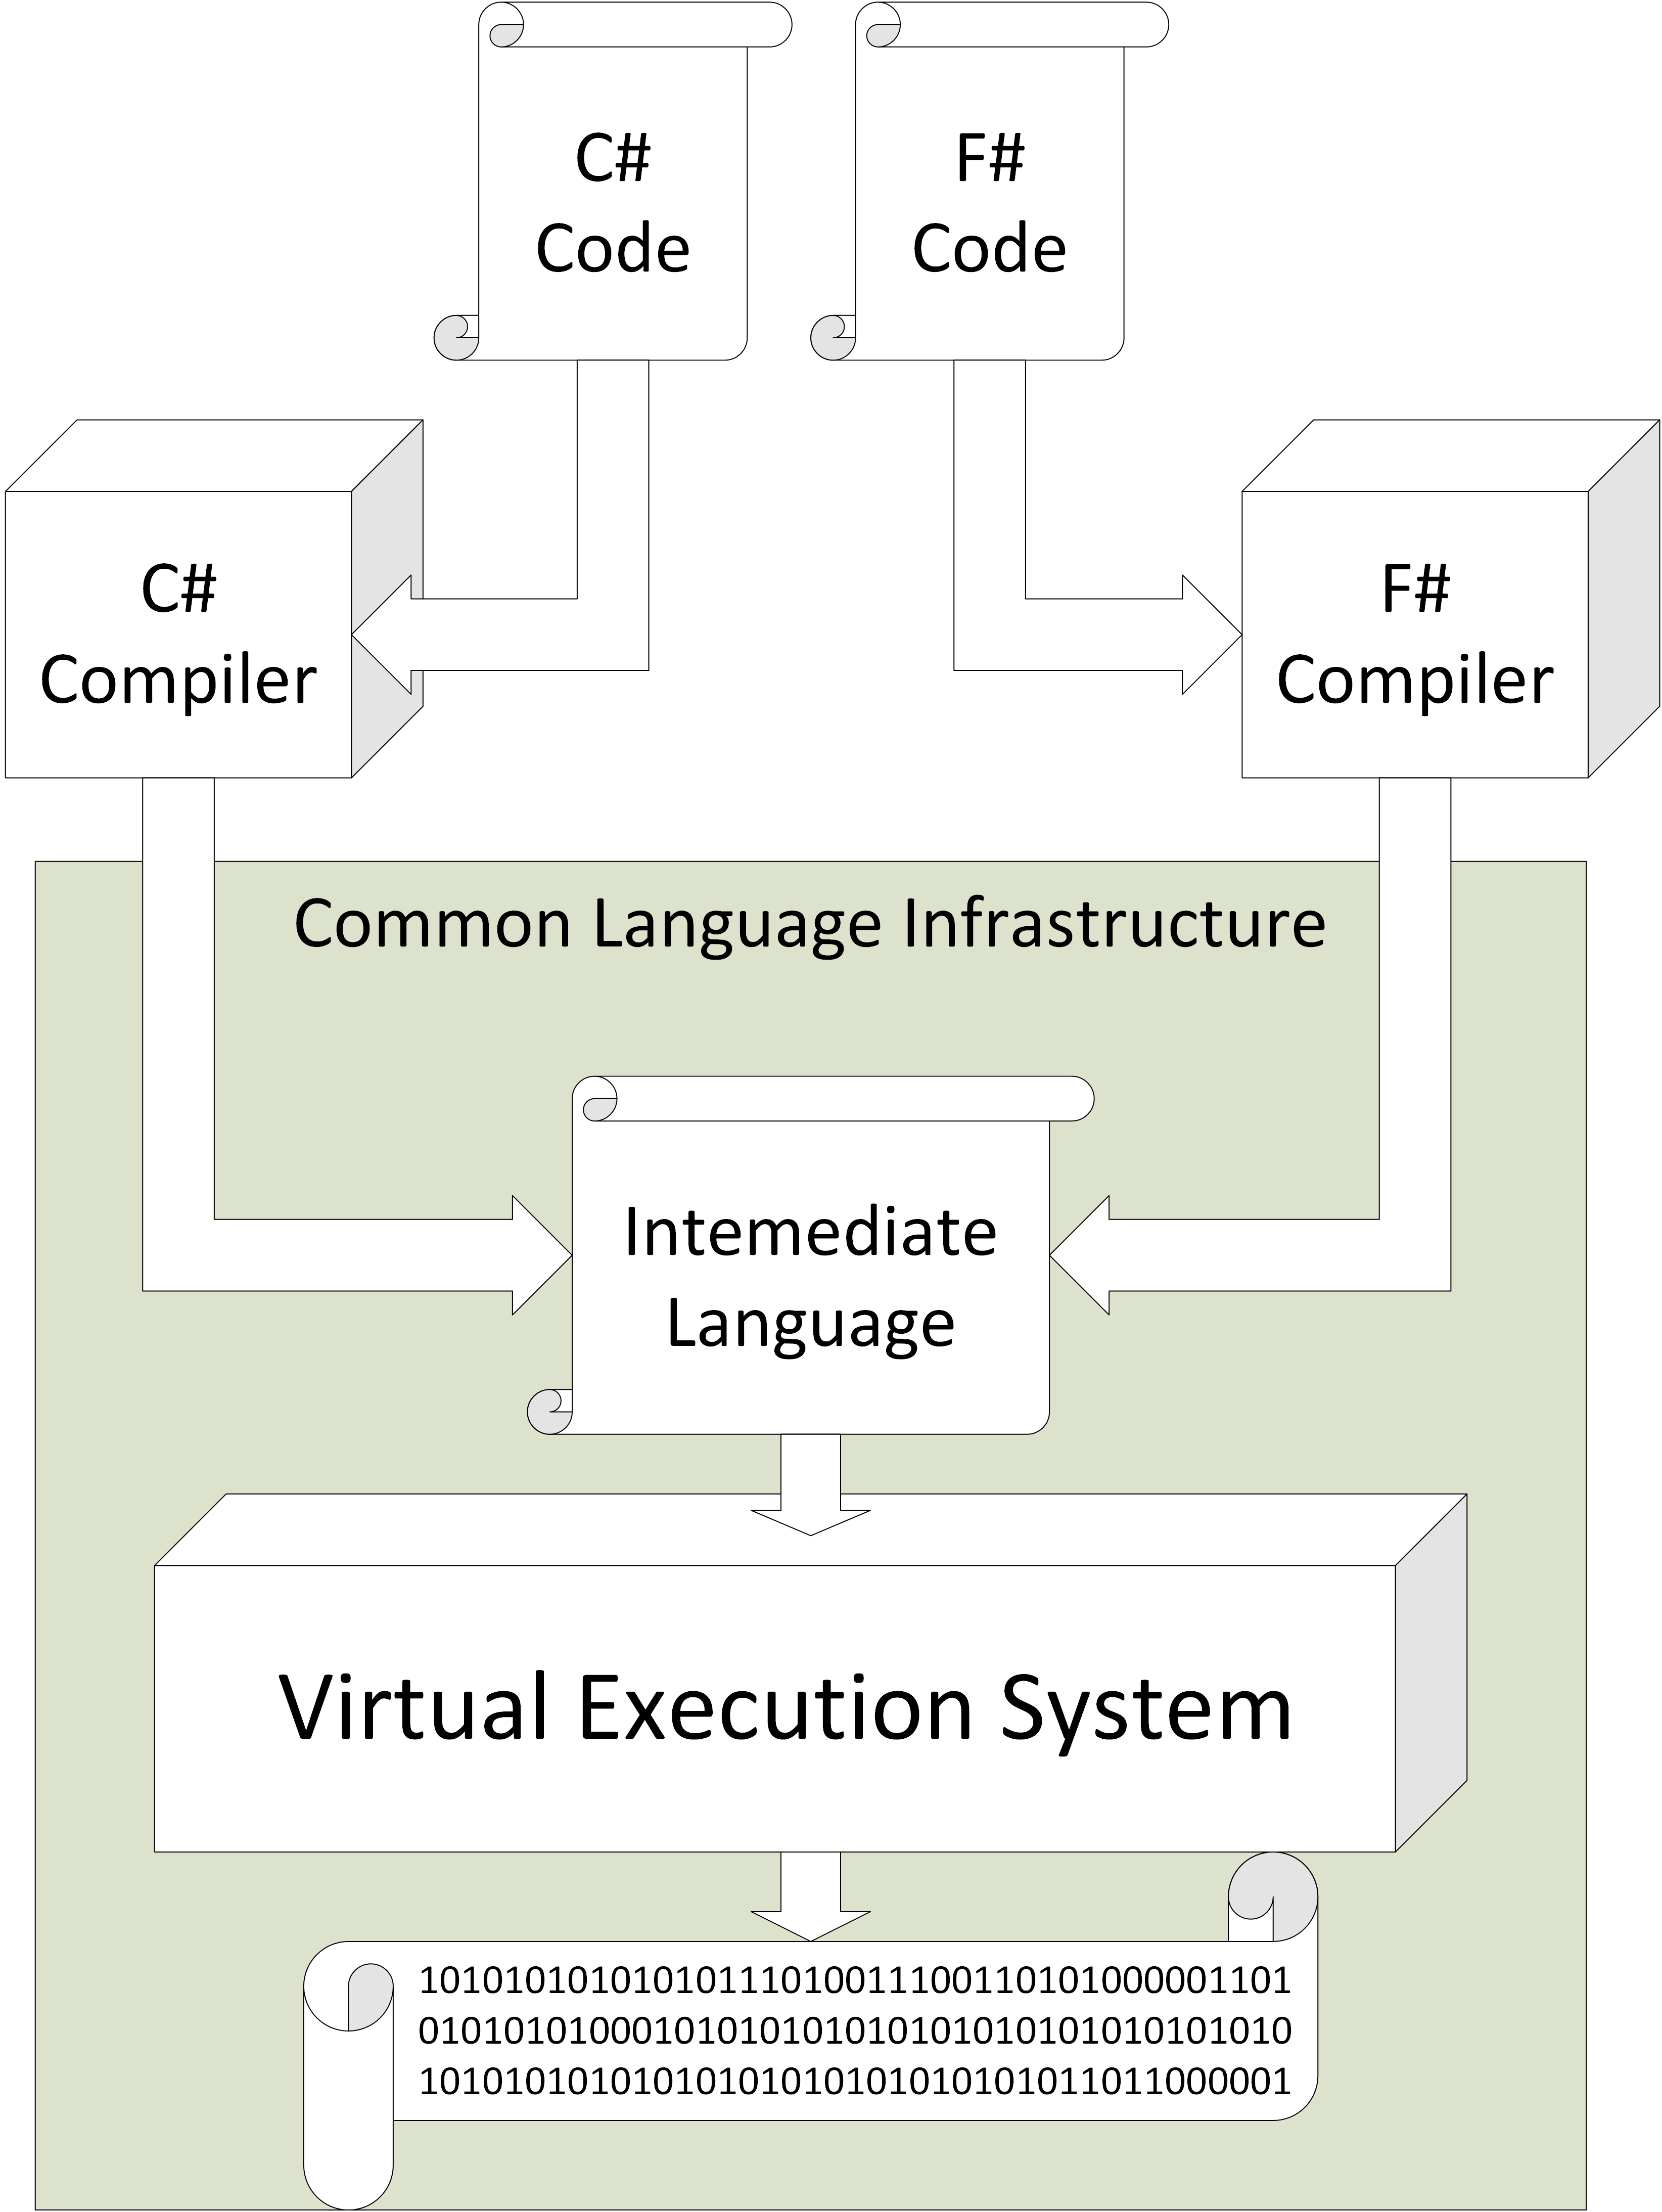
\includegraphics[width=1.0\textwidth]{CIL}
	\caption[CIL]{Common Language Infrastructure}
	\label{fig:CIL}
\end{figure}

La compilazione di un programma ad alto livello come può essere C# o F# viene tradotto in istruzioni di tipo Common Intermediate Language (CIL), un linguaggio intermedio indipendente dalla piattaforma, successivamente
come mostrato in \figurename~\ref{fig:CIL},  un VES specifico per la piattaforma traduce le istruzioni CIL in linguaggio macchina, un linguaggio direttamente comprensibile dal processore della piattaforma.

Il progetto Mono implementa sia VES per l'esecuzione dei programmi .NET per diverse piattaforme che compilatori per diversi linguaggi di programmazione, tra le VES implementate c'è anche quella per Linux per processori x64 ARM e tra i compilatori di linguaggi implemetanti da Mono c'è sia il compilatore per \texttt{C\#} che quello per \texttt{F\#} che verrano utilizzati in questo progetto.

Nell'appendice A sarà  descritto come installare Mono e il compilatore \texttt{F\#} su Rpi3.

\section{\texttt{Raspberry\#}}
Nel progetto utilizzerò due librerie rilasciate dalla comunity \texttt{Raspberry\#}  che consentono di utilizzare le funzionalità di Raspberry in ambiente .Net/Mono, quindi utilizzabili sia con il linguaggio \texttt{C\#} che con \texttt{F\#}.



\begin{itemize}
\item Raspberry.IO.GeneralPurpose  contiene classi che permettono di accedere all'hardware GPIO, il cui accesso richiede elevati privilegi di esecuzione e per ottenerli, i programmi che utilizzeranno queste funzionalità dovranno essere seguiti, sotto Raspian, usando il comando sudo.
\item Raspberry.System offre delle funzionalità di utilità per la scheda Raspberry, come la rilevazione automatica della scheda e l'implementazione di timer ad alta risoluzione.
\end{itemize}


Per  accedere a basso livello all'hardware GPIO, utilizzeremo il namespace Raspberry.IO.GeneralPurpose ci fornisce tre driver di accesso all'intefaccia GPIO:
\begin{itemize}
\item \textbf{GpioConnectionDriver}: l'accesso ai pin GPIO avviene attraverso al loro indirizzo di memoria e  utilizza un meccanisco di pseudo-interreput per individuare il cambiamento di stato del pin,
\item \textbf{MemoryGpioConnectionDriver}: l'accesso ai pin GPIO avviene attraverso il loro indirizzo di memoria,
\item \textbf{FileGpioConnectionDriver}: Questa implementazione usa i file virtuali  per accedere ai pin GPIO.
\end{itemize}

Tutti questi oggetti sono implementanzioni dell'interfaccia \textbf{IGpioConnectionDriver}, che definisce i seguenti metodi:


 %  \begin{itemize}
 %  \item IGpioConnectionDriver:interfaccia e implementazioni che formiscono un accesso a basso livello all'hardware GPIO.
 % rilascio di risorse correlate.
  
  % \item GpioConnection, GpioConnectionSettings, PinConfiguration and  le classi correllate forniscono un accesso gestito ai pin di input/output
  %\itemLa classe PinsBehavior e le sue sottoclassi forniscono un modo per raggruppare più pin di output ed applicare un comportamento comune.%
%	\end{itemize}

%\paragraph{IGpioConnectionDriver}

   % Il IGpioConnectionDriver definisce un'interfaccia per i driver di connessione GPIO. Un driver di connessione gestire l'accesso ai ingresso (lettura) e di uscita (scrittura) pin GPIO, così come l'uso e il 
   
   
  %\paragraph{Methods}
   
   
  %\textbf{Allocate}
  
  
   \begin{lstlisting}[frame=none]
   void Allocate(ProcessorPin pin, PinDirection direction);
   \end{lstlisting}
    
   Alloca un pin: attiva il pin in base al numero di pin dato e la direzione.
   Prende come parametri:
   \begin{itemize}
  	 \item pin: il pin, così come numerato sul processore
  	 \item direction: la direzione del pin direction, può assumere valori PinDirection.Input o PinDirection.Output
	\end{itemize}
   


	\begin{lstlisting}[frame=none]
   void Release(ProcessorPin pin);
 	\end{lstlisting}
   
   Rilascia un pin; si smette di utilizzare il pin specificato nel parametro
 
   
 
      
  \begin{lstlisting}[frame=none]
   bool Read(ProcessorPin pin);
  \end{lstlisting}
  
   Legge lo stato corrente del pin di input specificato come parametre. Il valore di ritorno è un booleano e rappresenta lo stato del pin. 
  

\begin{lstlisting}[frame=none]
void Write(ProcessorPin pin, bool value);
\end{lstlisting}
Aggiorna lo stato del pin specificato con il valore dato. I suoi parametri:
\begin{itemize}
\item	pin: il pin
\item	value: il nuovo valore booleano del pin
\end{itemize}
 E' possibile anche utilizzare un maggiore livello di astrazione per poter interagire con l'hardware,
 utilizzando le estensioni del driver che implementa la IGpioConnectionDriver possiamo usare i metodi
   \begin{lstlisting}[frame=none]
 public static GpioOutputBinaryPin Out(this IGpioConnectionDriver driver, ProcessorPin pin)
 public static GpioInputBinaryPin In(this IGpioConnectionDriver driver, ProcessorPin pin, PinResistor resistor = PinResistor.None)
 \end{lstlisting}
che consentono di ottenere oggetti, partendo dal ProcessorPin, che implementano rispettiva IOutputBinaryPin, IInputBinaryPin.

Su quest'ultima interfaccia è presente una funzionalità che sarà molto utile per utilizzare il sensore HC-SR04:

\begin{lstlisting}[frame=none]
public static TimeSpan Time(this IInputBinaryPin pin, bool waitForUp = true, TimeSpan phase1Timeout = new TimeSpan(), TimeSpan phase2Timeout = new TimeSpan())

\end{lstlisting}
Questo metodo attende che un pin raggiunga un terminato stato, quindi misura il tempo che rimane in questo stato, i suoi parametri sono:
\begin{itemize}
	 \item pin: il pin da misurare,
	 \item waitForUp: se è impostato a true, aspetta che il pin sia in High.
	 \item il timeout della prima fase
	 \item il timeout della seconda fase.
\end{itemize}
Il valore di ritorno è la durata dell'intervallo tra le due fasi, quindi il tempo che il pin rimane in High.
  
Infine nel package Raspberry.System utilizzero il metodo statico
\begin{lstlisting}[frame=none]
Timer.Sleep(TimeSpam)
\end{lstlisting}
che implementa un timer ad alta risoluzione.


\section{Node.js}

Node.js è un ambiente di esecuzione Javascript  opensource ed è disponibile su molte architetture, la piattaforma Node.js è basata sul Javascript Engine V8 di Google.
La principale caratteristica di Node.js è la sua  architettura event-driver per le I/O asincrone.
Inoltre offre anche un sistema di gestione dei pacchetti chiamato npm che permette di  in modo semplice e veloce di scaricare, installare e di integrare nel proprio progetto funzionalità aggiuntive offerte da moduli realizzati da una grandissima comunità.
Nel progetto utilizzero alcuni di questi pacchetti disponibili dal repository ufficale.


\subsection{Express.js}
Express.js è un framework per Node.js utile per implementare web application ed per creare API REST per servizi. 
\subsection{Telegram.js}
L’idea del progetto è di poter interagire con il robot con un I messaggistica, la scelta è caduta su telegram perché consente in maniera semplice di realizzare bot e interagirci attraverso API REST con risultanti in JSON. Nel repository Npm è presente il pacchetto Telegram.js che consente in modo semplice di integrare un applicazione node con le funzionalità offerte da telegram.

L'appendice E mostro come configurare Node.js per le funzionalità telegram

\section{Microsoft Cognitive Services} 
Cognitive Services (anche noto con il nome di Project Oxford) è un insieme di servizi esposti come API REST che permettono di aggiungere alle nostre applicazioni delle funzionalità “cognitive”, cioè funzionalità che abilitano le nostre applicazioni alla “comprensione” del mondo che le circonda. Nel progetto utilizzero i servizi cognitive Service che sono nella categoria Vision Service  che permettono di analizzare immagini o video alla ricerca di informazioni. 



\section{$ \texttt{ML}_{CoDa} $}
$ \texttt{ML}_{CoDa} $ è un linguaggio di programmazione orientanto al contesto. Questo linguaggio consente con alcuni costrutti di adattare il programma al contesto in cui viene eseguito. Il prototipo del linguaggio $ \texttt{ML}_{CoDa}} $ che userò è un estensione del linguaggio funzionale F#, della famiglia dei linguaggi ML.


Il contesto è l'ambiente dove le applicazioni vengono eseguite è un concetto fondamentale per il software adattivo. Il contesto può essere diviso in due parti: il contesto di sistema e il contesto applicativo.
Il contesto di sistema è la parte indipendente l'applicazione ad esempio l'hardware su cui viene esecutivo l'applicativo e l'ambiente fisico con il sistema può interagire.
il contesto applicativo è quello dipendente dall'applicazione come possono essere configurazioni utente.

Entrambi le parti in $ \texttt{ML}_{CoDa} $ sono rappresentati e gestiti in maniera omogenea. Questo linguaggio offre due componenti: una dichiarativa e una funzionale.

La componente dichiarativa  utilizza il DataLog per definire una base di conoscenza sulla quale i programmi adattivi possono interrogare il contesto e recuperare le informazioni che hanno bisogno.
Il datalog permette di definre regole che secondo la forma
Ogni regola è composta da una testa (head o LHS) e 
da un corpo (body o RHS)
p :- p1, p2, ... pn
•
Ogni P rappresenta un predicato (chiamato 
letterale), così composto:

•nome
•argomenti:
•
costanti
•
variabili
•
simbolo “don’t care” ( _ ) (non nella testa)
• Le variabili del LHS devono apparire nel RHS
negazione

La componente funzionale  estende F# con alcune istruzioni che hanno lo scopo per poter interrogare e modificare con la base informativa definita in Prodata,
retract <|
tell <|

 le istruzioni sono
 
 Goal ctx?exam
 
 let x = expression1 |- Goal [in] expression2
 
 for _ in !-- Goal do expression
 
 match ctx with | _ when !- Goal -> expression
 
 per poter usare queste istruzioni è necessario marcare il codice con alcune annotazioni
 
 The application programmer writes F# code, annotating the functions which use MLCoDa extensions with custom attributes and starting the MLCoDa runtime. 
 Since the operations needed to adapt the application to contexts are transparently handled by our runtime support, the compiler fsharpc works as it is. 
 Indeed, the MLCoDa-specific constructs are just-in-time replaced in a single step by their F# implementation when they are about to be run. A simple example follows.
 Actually, the attribute CoDa.Code is an alias for the standard ReflectedDefinitionAttribute, that marks modules and members whose abstract syntax trees (AST) are used at runtime through reflection. 
 Note that MLCoDa-specific operations are only allowed in methods marked with this attribute; 
 otherwise an exception is raised when they are invoked The attribute CoDa.EntryPoint marks the principal function of the application (main above). 
 
 
 When the MLCoDa runtime is initialised and started through the function run, it looks for the function f marked by CoDa.EntryPoint; then it transforms the code of the function replacing the MLCoDa-specific constructs with their F# object code;  
 and finally runs the obtained object code. The translation is performed on the AST represented in the form of quotations. Hereafter, for readability, we will show the object code in F# syntax, rather than the quotation emitted by the JIT compiler.
 [<CoDa.Code>]
 
 [<CoDa.ContextInit>]
 
 [<CoDa.Context("fsc-ctx")>]
 
 [< CoDa.EntryPoint>]
 

L'appendice F descrivo la catena di compilazione di programma adattivo di esempio che utilizza $ \texttt{ML}_{CoDa} $ in modo da mostrare quali strumenti software sono utilizzati per questo progetto.


 
Nell'appendice D descrivo come testare gli esempi di $ \texttt{ML}_{CoDa} $ su Mono installato su Rpi3
 
Nell'appendice E implemento il progetto button-led in $ \texttt{ML}_{CoDa} $



